\documentclass[12pt,a4paper]{article}
\usepackage{geometry}
\geometry{left=2.5cm,right=2.5cm,top=2.0cm,bottom=2.5cm}
\usepackage[english]{babel}
\usepackage{amsmath,amsthm,mathtools}
\usepackage{amsfonts}
\usepackage[longend,ruled,linesnumbered]{algorithm2e}
\usepackage{fancyhdr}
\usepackage{ctex}
\usepackage{array}
\usepackage{listings}
\usepackage{color}
\usepackage{graphicx}
\usepackage{amssymb}
\newtheorem{theorem}{定理}
\newtheorem{lemma}[theorem]{引理}
\newtheorem{corollary}[theorem]{推论}

\begin{document}
	
	\noindent
	
	\section*{2024.04.08}	
	
	
	\begin{enumerate}
		\item 利用$Young$不等式证明$H\ddot{o}lder$不等式.
		
		\begin{theorem}{($Young$不等式)}
			
			设 $p>1, q>1$, 且 $\frac{1}{p}+\frac{1}{q}=1$, 则对 $\forall a, b \geq 0$, 有
			\begin{equation} 
				a b \leq \frac{a^p}{p}+\frac{b^q}{q} .\label{young}
			\end{equation}
		\end{theorem}
		
		\begin{theorem}{($H\ddot{o}lder$不等式)}
			
			对 $f \in L^p(\Omega), g \in L^q(\Omega), 1 \leqslant p, q \leqslant+\infty, \frac{1}{p}+\frac{1}{q}=1$, 有
			\begin{equation}
				\|f g\|_{0,1, \Omega} \leqslant\|f\|_{0, p, \Omega}\|g\|_{0, q, \Omega} .\label{holder}
			\end{equation}
			
			
		\end{theorem}
		
		\begin{proof}
			
			若 $\|f\|_{0, p, \Omega}=0$ (或 $\|g\|_{0, q, \Omega}=0$), 则$f(\boldsymbol{x}) = 0$(或 $g(\boldsymbol{x})=0$), a.e. $\boldsymbol{x} \in \Omega$, 进而 $f(\boldsymbol{x}) g(\boldsymbol{x})=0$, a.e. $\boldsymbol{x} \in \Omega$, 此时 \eqref{holder}左侧与右侧均为0, 成立.
			
			否则 $\|f\|_{0, p, \Omega} \neq 0,\|g\|_{0, q, \Omega} \neq 0$. 取 $a=\frac{|f(\boldsymbol{x})|}{\|f\|_{0, p, \Omega}}, b=\frac{|g(\boldsymbol{x})|}{\|g\|_{0, q, \Omega}}$, 代入 \eqref{young}式后两边在 $\Omega$ 上积分, 得到 
			
			\begin{equation*}
				\begin{aligned}
					\int_{\Omega}\frac{|f(\boldsymbol{x})|}{\|f\|_{0, p, \Omega}}\frac{|g(\boldsymbol{x})|}{\|g\|_{0, q, \Omega}} dx &\leq \frac{1}{p} \frac{\int_{\Omega}|f(\boldsymbol{x})|^p dx}{\|f\|_{0, p, \Omega}^p} + \frac{1}{q} \frac{\int_{\Omega}|g(\boldsymbol{x})|^q dx}{\|g\|_{0, q, \Omega}^q}\\
					& = \frac{1}{p}+\frac{1}{q}\\
					& = 1
				\end{aligned} 
			\end{equation*}
			整理即得\eqref{holder}.
			
		\end{proof}
		
		\item 证明$W^{1,p}$是Banach空间.(利用$L^p$完备)
		
		\begin{proof}
			
			直接证明$W^{m,p}$是Banach空间.只要证明 $W^{m, p}(\Omega)$ 在Sobolev范数下是完备的.
			
			令 $\left\{v_j\right\} \subset W^{m, p}(\Omega)$ 是 Cauchy 列, 即 $\left\{D^\alpha v_j:|\alpha| \leq m\right\}$ 是 $L^p(\Omega)$ 中的 Cauchy 列. 由于 $L^p(\Omega)$ 是完备的, 从而存在 $v_\alpha \in L^p(\Omega)(|\alpha| \leq$ $m)$, 使得 $D^\alpha v_j \rightarrow v_\alpha$ 在 $L^p(\Omega)$ 中, 当 $j \rightarrow \infty$ 时. 余下只要证明 $v_\alpha=D^\alpha v$, 即 $\forall \varphi \in C_0^{\infty}(\Omega)$ ,
			$$
			\int_{\Omega} v_\alpha \cdot \varphi d x=(-1)^{|\alpha|} \int_{\Omega} v \cdot \partial^\alpha \varphi d x .
			$$
			
			事实上,
			$$
			\begin{aligned}
				\int_{\Omega} v_\alpha \cdot \varphi d x & =\lim _{j \rightarrow \infty} \int_{\Omega} D^\alpha v_j \cdot \varphi \mathrm{d} x \\
				& =\lim _{j \rightarrow \infty}(-1)^{|\alpha|} \int_{\Omega} v_j \cdot \partial^\alpha \varphi d x=(-1)^{|\alpha|} \int_{\Omega} v \cdot \partial^\alpha \varphi d x.
			\end{aligned}
			$$
		\end{proof}
		
		\item 设 $\Omega=(-1,1)$ ,
		$$
		f(x)=|x|= \begin{cases}x, & 0 \leq x<1 \\ -x, & -1<x<0\end{cases}
		$$
		
		证明
		$$
		g(x)= \begin{cases}1, & 0<x<1 \\ -1, & -1<x<0\end{cases}
		$$
		
		是 $f$ 的一阶广义导数.
		
		\begin{proof}
			$\forall \varphi \in C_0^{\infty}(\Omega)$, 由分部积分,
			$$
			\begin{aligned}
				\int_{-1}^1 f(x) \cdot \varphi^{\prime}(x) \mathrm{d} x & =\int_{-1}^0 f(x) \cdot \varphi^{\prime}(x) \mathrm{d} x+\int_0^1 f(x) \cdot \varphi^{\prime}(x) \mathrm{d} x \\
				& =\int_{-1}^0 \varphi(x) \mathrm{d} x-\int_0^1 \varphi(x) \mathrm{d} x \\
				& =-\int_{-1}^1 g(x) \varphi(x) \mathrm{d} x
			\end{aligned}
			$$
			
			其中
			$$
			g(x) = \begin{cases}1, & 0<x<1 \\ -1, & -1<x<0\end{cases}
			$$
			
			显然$g$是局部Lesbegue可积函数,故$g$是$f$的一阶广义导数.
		\end{proof}
		
		\item 推导Poisson方程的混合边值问题
		\begin{equation} 
			\left\{\begin{array}{l}
				-\Delta u=f, \text { 在 } \Omega \text { 内 } \\
				\left.u\right|_{\Gamma_1}=g_1 \\
				\left.\frac{\partial u}{\partial n}\right|_{\Gamma_2}=g_2
			\end{array}\right. \label{Possion}
		\end{equation}
		
		
		
		的变分形式, 这里 $\partial \Omega=\Gamma_1 \cup \Gamma_2$, 且 $\Gamma_1 \cap \Gamma_2=\emptyset$. 并证明古典解和弱解在一定条件下等价.
		
		\begin{proof}[解]\let\qed\relax
			设$V = \{v\ | v \in H^1(\Omega), \left.v\right|_{\Gamma_1} = 0\}$.
			
			对任意 $v \in V$, 用Green公式可得
			$$
			\begin{aligned}
				& \int_{\Omega} \nabla u \cdot \nabla v \mathrm{dx}-\int_{\Gamma_2} \frac{\partial u}{\partial n} v \mathrm{ds}=\int_{\Omega} f v \mathrm{dx} \\
				& \Rightarrow \int_{\Omega} \nabla u \cdot \nabla v \mathrm{dx}=\int_{\Omega} f v \mathrm{dx}+\int_{\Gamma_2} g_2 v \mathrm{ds}
			\end{aligned}
			$$
			
			则问题\eqref{Possion}的变分形式是: 求 $u \in H^1(\Omega)$且$\left.u\right|_{\Gamma_1} = g_1$ 使得
			\begin{equation}
				a(u, v)=(f, v)+\int_{\Gamma_2} g_2 v \mathrm{ds}, \quad \forall v \in V.
				\label{weak}
			\end{equation}
			
			
			
		\end{proof}
		
		\begin{theorem}
			设 $f \in C(\overline{\Omega}), g_1,g_2  \in C(\partial \Omega)$. 如果 $u \in C^2(\overline{\Omega})$ 是问题\eqref{Possion}的古典解, 则它是弱解. 反过来, 如果 $u$ 是问题\eqref{Possion}的弱解且 $u \in C^2(\overline{\Omega})$, 则它是古典解.
		\end{theorem}
		
		\begin{proof}
			第一个结论显然. 
			
			如果 $u$ 是问题\eqref{Possion}的弱解且 $u \in C^2(\overline{\Omega})$,立得$\left.u\right|_{\Gamma_1}=g_1$.
			
			第一步在\eqref{weak}中取 $v \in C_0^{\infty}(\Omega)$, 利用Green公式和 $\left.v\right|_{\partial \Omega}=0$ 得到
			$$
			\int_{\Omega}(\Delta u+f) v \mathrm{dx}=0 .
			$$
			
			推出 $\Delta u+f=0$. 第二步在(4)中取 $v \in C^{\infty}(\overline{\Omega})$且$\left.v\right|_{\Gamma_1} = 0$, 注意到 $\Delta u+f=0$, 可得
			$$
			\int_{\Gamma_2} \frac{\partial u}{\partial n} v \mathrm{ds}=\int_{\Gamma_2} g_2 v \mathrm{ds}
			$$
			
			由 $v$ 的任意性得到 $u$ 满足边界条件 $\left.\frac{\partial u}{\partial n}\right|_{\Gamma_2}=g_2$.
			
			三个条件均满足,故 $u$ 是古典解.
		\end{proof}
	\end{enumerate}
	
	
	\newpage
	
	\section*{2024.04.15}	
	
	
	\begin{enumerate}
		\item 推导		
		$
		\displaystyle \int_\Omega v\Delta^2u\mathrm{~dx}-\displaystyle \int_\Omega\Delta u\Delta v\mathrm{~dx}
		$
		边界项
		
		\begin{proof}[解]\let\qed\relax
			给定 $u,v\in H^1(\Omega)$, 根据Green 公式:对 $1\leqslant i\leqslant n$,
			\begin{equation}
				\int_{\Omega}u\partial_{i}v\mathrm{d}\boldsymbol{x}=-\int_{\Omega}v\partial_{i}u\mathrm{d}\boldsymbol{x}+\int_{\Gamma}uvn_{i}\mathrm{d}s\label{green1}
			\end{equation}
			
			若$u\in H^2(\Omega),\quad v\in H^1(\Omega)$,则可用 $\partial_{i}u$ 代替\eqref{green1}式中的 $u$,可得
			
			$$
			\int_{\Omega}\partial_{i}u\partial_{i}v\mathrm{d}\boldsymbol{x}=-\int_{\Omega}v\partial_{ii}u\mathrm{d}\boldsymbol{x}+\int_{\Gamma}\partial_{i}uvn_{i}\mathrm{d}s
			$$
			
			对 $i$ 从 1 到 $n$ 求和可得
			\begin{equation}
				\int_{\Omega}\nabla u\nabla v\mathrm{d}\boldsymbol{x}=-\int_{\Omega}v\Delta u\mathrm{d}\boldsymbol{x}+\int_{\Gamma}v\frac{\partial u}{\partial n}\mathrm{d}s\label{green2}
			\end{equation}
			
			若$v\in H^2(\Omega),\quad u\in H^1(\Omega)$,类似地有
			\begin{equation}
				\int_{\Omega}\nabla u\nabla v\mathrm{d}\boldsymbol{x}=-\int_{\Omega}u\Delta v\mathrm{d}\boldsymbol{x}+\int_{\Gamma}u\frac{\partial v}{\partial n}\mathrm{d}s\label{green3}
			\end{equation}
			
			则当$u, v\in H^2(\Omega)$,\eqref{green2}\eqref{green3}两式相减,得:
			\begin{equation}
				\int_{\Omega}\big(u\Delta v-v\Delta u\big)\mathrm{d}\boldsymbol{x}=\int_{\Gamma}\big(u\frac{\partial v}{\partial n}-v\frac{\partial u}{\partial n}\big)\mathrm{d}s,\forall u,v\in H^{2}(\Omega)\label{green4}
			\end{equation}
			
			若$u\in H^{4}(\Omega),v\in H^{2}(\Omega).$, 则可用 $\Delta u$ 代替\eqref{green4}中的 $u$, 可得
			
			$$
			\int_\Omega\Delta u\Delta v\mathrm{d}\boldsymbol{x}=\int_\Omega v\Delta^2u\mathrm{d}\boldsymbol{x}-\int_\Gamma v\frac{\partial\Delta u}{\partial n}\mathrm{d}s+\int_\Gamma\Delta u\frac{\partial v}{\partial n}\mathrm{d}s
			$$
			
		\end{proof}
		
		\item 
		当双线性型$a(\cdot,\cdot)$对称时,利用$a(\cdot,\cdot)$可定义$V$上的新内积和Riesz表示定理证明Lax-Milgram定理(根据注的提示)
		
		\begin{theorem}(Lax-Milgram 定理)
			
			设$V$ 是一个 Hilbert 空间,$a(u,v)$ 是$V\times V$ 上的对称、连续、强制的双线性形式,$f$ 是$V$ 中的线性连续泛函,则变分问题
			$$\text{求 }u\in V,\text{ 使得 }a(u,v)=\langle f,v\rangle,\quad\forall v\in V,$$
			
			存在唯一解$u^*$,且满足范数估计
			
			$$
			\left\|u^*\right\|_V\leqslant\frac{1}{\alpha}\left\|f\right\|_{V^*},
			$$
			
		\end{theorem}
		
		\begin{proof}
			因 $a(u,v)$ 是对称、正定的,故可在$V$ 上定义新内积 $[u,v]\triangleq a(u,v)$, 且
			
			$$
			\alpha{\left\|u\right\|}_{V}^{2}\leqslant\left[u,u\right]\leqslant M{\left\|u\right\|}_{V}^{2},
			$$
			
			其中左侧由强制性,右侧由连续性.
			
			新定义的内积所确定的范数 $\sqrt{a(u,u)}$ 与范数 $\|\cdot\|_V$ 等价. 对于 $V$ 的新范数$\sqrt{a(u,u)}$ 而言 $f$ 仍是线性连续泛函. 根据 Riesz 表示定理可知,存在唯一的 $u^*\in V$ 使得
			
			$$
			[u^*,v]=\left\langle f,v\right\rangle,\quad\forall\:v\in V,
			$$
			
			即
			
			$$
			a(u^*,v)=\langle f,v\rangle,\quad\forall\:v\in V.
			$$
			
			于是 $u^*$ 就是变分问题的唯一解.另一方面
			
			$$
			\alpha\|u^*\|_V^2\leqslant a(u^*,u^*)=[u^*,u^*]=\langle f,u^*\rangle\leqslant\|f\|_{V^*}\|u^*\|_V.
			$$
			
			从而得到范数估计.
		\end{proof}
		
		\item 证明Poincaré不等式
		\begin{equation}
			\|v\|_{m,\Omega}^2\leq C_2\Big(|v|_{m,\Omega}^2+\sum_{|\alpha|<m}\Big(\int_\Omega\partial^\alpha v\mathrm{dx}\Big)^2\Big),\forall v\in H^m(\Omega),\label{poincare}
		\end{equation}
		
		\begin{proof}
			利用反证法. 假设\eqref{poincare}不成立. 对每个正整数$k$, 存在$v_k\in H^m(\Omega)$使
			
			$$
			\|v_k\|^2_{m,\Omega}>k\Big(|v_k|_{m,\Omega}^2+\sum_{|\alpha|<m}\Big(\int_\Omega\partial^\alpha v_k\mathrm{dx}\Big)^2\Big).
			$$
			
			不失一般性,设$v_k$满足
			
			$$
			\left\|v_k\right\|_{m,\Omega}=1,\:k=1,2,\cdots,
			$$
			
			这样有
			
			$$
			\lim_{k\to\infty}|v_k|_{m,\Omega}=0.
			$$
			$$
			\lim_{k\to\infty}\int_\Omega\partial^\alpha v_k\mathrm{dx} = 0, \quad \forall \alpha \quad s.t. |\alpha|<m
			$$
			
			因为$\{v_k\}$是$H^m(\Omega)$的有界序列,所以存在$v_\infty\in H^m(\Omega)$和一个子列(仍记为$\{v_k\})$满足:$\{v_k\}$弱收敛于$v_\infty$. 利用嵌入定理$H^m(\Omega)\overset{c}{\operatorname*{\hookrightarrow}}H^{m-1}(\Omega)$,
			在$H^{m-1}(\Omega)$中$\{v_k\}$强收敛于$v_{\infty}.$
			
			于是
			
			$$
			\lim_{k,\ell\to\infty}\|v_k-v_\ell\|_{m,\Omega}\leq\lim_{k,\ell\to\infty}\left(\|v_k-v_\ell\|_{m-1,\Omega}+|v_k-v_\ell|_{m,\Omega}\right)=0.
			$$
			因此$\{v_k\}$是$H^m(\Omega)$中的Cauchy序列,进而$\{v_k\}$在$H^m(\Omega)$中强收敛于$v_\infty.$ 由极限得到$\|v_\infty\|_{m,\Omega}=1$和$|v_\infty|_{m,\Omega}=0$, 即$v_{\infty}$是一个$m-1$次多项式. 
			
			注意到
			$$
			\int_\Omega\partial^\alpha v_\infty \mathrm{dx} = 0, \quad \forall \alpha \quad s.t. \ |\alpha|<m
			$$,
			
			可得$v_\infty\equiv0$.与$v_\infty\neq0$矛盾.上面讨论可推出Poincaré不等式成立.
			
			
		\end{proof}
		
		\item 考虑Robin边值问题
		\begin{equation}
			\begin{cases}-\Delta u+\alpha(x)u=f,\text{ 在}\Omega \text{上}\\(\frac{\partial u}{\partial n}+\beta(x)u)\left.\right|_{\partial\Omega}=g&\end{cases}
			\label{robin}
		\end{equation}
		
		
		这里$\alpha(x)\geq\alpha_0>0,\beta(x)\geq0$以及$f$均为足够光滑的已知函数
		
		\begin{enumerate}
			\item[(i)]   试建立该边值问题的变分问题
			\item[(ii)]  讨论变分问题解的存在唯一性(适定性)
		\end{enumerate}
		\begin{proof}[解]\let\qed\relax
			\begin{enumerate}
				\item[(i)] 
				
				对任意 $v \in H^1(\Omega)$, 用Green公式可得
				$$
				\begin{aligned}
					& \int_{\Omega} \nabla u \cdot \nabla v + \alpha(x)uv \mathrm{dx}-\int_{\partial \Omega} \frac{\partial u}{\partial n} v \mathrm{ds}=\int_{\Omega} f v \mathrm{dx} \\
					& \Rightarrow  \int_{\Omega} \nabla u \cdot \nabla v + \alpha(x)uv \mathrm{dx}+\int_{\partial \Omega}\beta(x)uv \mathrm{ds}=\int_{\Omega} f v \mathrm{dx} + \int_{\partial \Omega} gv \mathrm{ds}
				\end{aligned}
				$$
				
				则问题\eqref{robin}的变分形式是: 求 $u \in H^1(\Omega)$ 使得
				\begin{equation}
					a(u, v)=(f, v)+\int_{\partial \Omega} gv \mathrm{ds}, \quad \forall v \in V.
					\label{weak2}
				\end{equation}
				
				其中$a(u, v):= \int_{\Omega} \nabla u \cdot \nabla v + \alpha(x)uv \mathrm{dx}+\int_{\partial \Omega}\beta(x)uv \mathrm{ds}$.
				
				\item[(ii)] 只需要验证Lax-Milgram定理的条件:
				\begin{equation*}
					\begin{aligned}
						a(u,u) &= \int_{\Omega} (\nabla u)^2 + \alpha(x)u^2 \mathrm{dx}+\int_{\partial \Omega}\beta(x)u^2 \mathrm{ds}\\
						&\geqslant \int_{\Omega} (\nabla u)^2 + \alpha(x)u^2 \mathrm{dx}\\
						&\geqslant \min\{1,\alpha_0\} \|u\|_{1,\Omega}^2
					\end{aligned}
				\end{equation*}
				从而$a(u,v)$满足强制性
				
				\begin{equation*}
					\begin{aligned}
						|a(u,v)|&\leqslant\left|u\right|_{1,\Omega}\cdot\left|v\right|_{1,\Omega}+\sup_{\boldsymbol{x}\in\Omega}\alpha(\boldsymbol{x})\cdot\left\|u\right\|_{0,\Omega}\cdot\left\|v\right\|_{0,\Omega}+\sup_{\boldsymbol{x}\in\Omega}\beta(\boldsymbol{x})\cdot\left\|u\right\|_{0,\partial \Omega}\cdot\left\|v\right\|_{0,\partial \Omega}\\
						&\leqslant (1+\sup_{\boldsymbol{x}\in\Omega} \alpha(\boldsymbol{x})+\sup_{\boldsymbol{x}\in\Omega} \beta(\boldsymbol{x}))\|u\|_{1,\Omega}\cdot\|v\|_{1,\Omega},\quad\forall u,v\in V
					\end{aligned}
				\end{equation*}
				其中上式第一行用到了柯西积分不等式,第二行用到了范数性质以及迹定理.从而$a(u,v)$满足连续性.
				$$
				\left|\int_\Omega fv\mathrm{dx}\right|\leq\left\|f\right\|_{0,\Omega}\left\|v\right\|_{0,\Omega}\leq\left\|f\right\|_{0,\Omega}\left\|v\right\|_{1,\Omega}
				$$
				$$
				\left|\int_{\Omega}gv\mathrm{ds}\right|\leq\left\|g\right\|_{0,\partial\Omega}\left\|v\right\|_{0,\partial\Omega}\leq C\left\|g\right\|_{0,\partial\Omega}\left\|v\right\|_{1,\Omega}
				$$
				从而得到右端泛函有界性.
				
				综上,利用Lax-Milgram定理,变分问题\eqref{weak2}的解存在且唯一.
			\end{enumerate}
		\end{proof}
		
	\end{enumerate}
	\newpage
	
	\section*{2024.04.22}	
	
	\begin{enumerate}
		\item 证明如下引理.
		
		设$P_k$是$d$维空间,$\{N_1,\cdots,N_L\}$是$P_k$的对偶空间$(P_k)^{\prime}$的一个子集. 则下面两个条件等价
		
		(a) $\{N_1,\cdots,N_d\}$是$(P_k)^{\prime}$的一组基
		
		(b) 对任意$\phi\in P_K$,$N_i(\phi)=0,1\leq i\leq d$等价于$\phi\equiv0.$
		
		\begin{proof}
			令 $\{\phi_1, \ldots , \phi_d\} $ 为 $P_k$ 的一组基.$\left\{N_1,\ldots,N_d\right\}$ 是 $P_k^{\prime}$ 的一组基当且仅当对于 $\mathcal{P} ^{\prime}$ 中的任意 $L$,
			
			\begin{equation}
				L=\alpha_1N_1+\ldots+\alpha_dN_d  \label{linear}
			\end{equation}
			
			因为 $d= \dim P_k = \dim P_k ^{\prime}$. 式\eqref{linear}等价于
			
			\begin{equation}
				\begin{aligned}
					y_i &:= L(\phi_i) \\
					&= \alpha_1N_1(\phi_i)+\ldots+\alpha_dN_d(\phi_i),\quad i=1,\ldots,d.
				\end{aligned}
			\end{equation}
			
			
			令 $B=\left(N_j(\phi_i)\right),i,j=1,\ldots,d.$ 因此,(a) 等价于 $B\alpha=y$ 有解,即$B$可逆。
			
			对于 $\mathcal{P}$ 中的任意 $v$,我们可以写成 $v=\beta_1\phi_1+\ldots+\beta_d\phi_d.~N_iv=0$ 意味着 $\beta_1N_i(\phi_1)+\ldots+\beta_dN_i(\phi_d)=0.$ 因此,(b) 等价于
			
			\begin{equation}
				\beta_{1}N_{i}(\phi_{1})+\ldots+\beta_{d}N_{i}(\phi_{d})=0\quad\forall i=1,\ldots,d\\\Longrightarrow\beta_{1}=\ldots=\beta_{d}=0.
			\end{equation}
			
			令 $C=\begin{pmatrix}N_i(\phi_j)\end{pmatrix},\:i,j=1,\ldots,d.$ 那么 (b) 等价于 $Cx=0$ 只有零解,即$C$可逆。
			
			由于 $C=B^\top$, (a) 等价于 (b).
			
		\end{proof}
		\item 利用网格生成软件包给出L型区域$\Omega=(-1,1)^2\backslash[0,1]\times[-1,0]$的一个
		三角形剖分,画出剖分图(例如gmsh,distmesh等)
		
		\begin{figure}[ht]
			\centering
			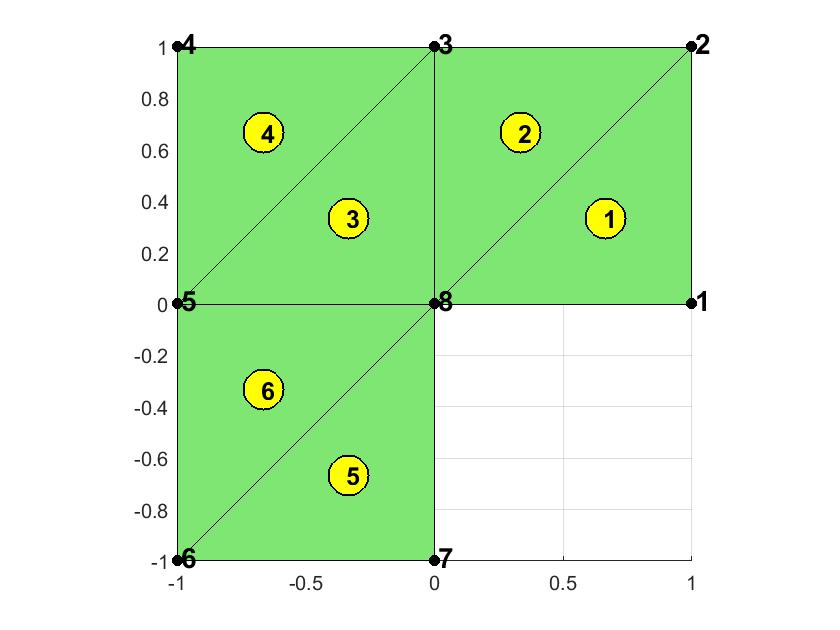
\includegraphics[width=0.8\textwidth]{hw3_2.jpg}
			\caption{网格图}
			\label{fig:triangelmesh}
		\end{figure}
		
		\item 验证
		$$
		\phi_i=\lambda_i(2\lambda_i-1),\quad1\leq i\leq3
		$$
		
		$$
		\phi_4=4\lambda_2\lambda_3,\:\phi_5=4\lambda_3\lambda_1,\:\phi_6=4\lambda_1\lambda_2
		$$
		
		是Lagrange二次元节点基函数. 
		
		\begin{proof}
			直接代入计算可得
			$$
			\phi_1(z_i)=\lambda_1(2\lambda_1-1)=0(2*0-1)=0, \quad i = 2,3,4
			$$
			$$
			\phi_1(z_i)=\lambda_1(2\lambda_1-1)=\frac{1}{2}(2*\frac{1}{2}-1)=0, \quad i = 5,6
			$$
			$$
			\phi_1(z_i)=\lambda_1(2\lambda_1-1)=1(2*1-1)=1, \quad i = 1
			$$
			$$
			\phi_4(z_i)=4\lambda_2\lambda_3=4*0*0=0, \quad i = 1
			$$
			
			$$
			\phi_4(z_i)=4\lambda_2\lambda_3=4*\frac{1}{2}*0=0, \quad i = 5,6
			$$
			
			$$
			\phi_4(z_i)=4\lambda_2\lambda_3=4*1*0=0, \quad i = 2,3
			$$
			
			$$
			\phi_4(z_i)=4\lambda_2\lambda_3=4*\frac{1}{2}*\frac{1}{2}=1, \quad i = 4
			$$
			由对称性以及Lagrange元定义,可得$N_i(\phi_j)=\delta_{ij}$,从而$\phi$是Lagrange二次元节点基函数
		\end{proof}
		
		\item 证明如下定义的Hermite空间属于$H^1(\Omega)$
		
		$$
		V_h=\{v\in L^2(\Omega)\mid v|_K\in P_3(K),\forall K\in \mathcal{T}_h,v\text{在}\mathcal{T}_h\text{的所有顶点连续},\nabla v\text{在}\mathcal{T}_h\text{的所有顶点连续}\}
		$$
		
		(Hint:要证$V_h\subset H^1(\Omega)$只需证在公共边$F=K_1\cap K_2$上,$v|_{K_1}=v|_{K_2})$
		
		\begin{proof}
			考虑$v|_{K_1}$与$v|_{K_2}$在$K_1\cup K_2$上的延拓,仍记为$v|_{K_1},v|_{K_2}$.
			
			记$w := v|_{K_1}-v|_{K_2}$,则$w$是定义在$K_1\cup K_2$上的$P_3$的多项式.
			
			记$L := K_1\cap K_2$的两个端点为$z_1,z_2$,根据$V_h$定义,有
			$$
			w(z_1)=w_(z_2)=0
			$$
			$$
			w_{L}^{\prime}(z_1)=w_{L}^{\prime}(z_2)=0
			$$
			从而有$w|_{L}\equiv0$. 即$v|_{K_1}=v|_{K_2}$
		\end{proof}
		
		\item 证明如下定义的Argyris空间属于$H^2(\Omega)$ 
		$$V_h=\{v\in L^2(\Omega)\mid v|_K\in P_5(K),\forall K\in \mathcal{T}_h,v\text{和其一阶以及二阶导数在}\mathcal{T}_h
		\text{的所有顶点连续,在}$$
		$$\mathcal{T}_h\text{的所有边中点,}v\text{关于该边的法向导数连续}\}$$
		
		(Hint:要证$V_h\subset H^2(\Omega)$只需证在公共边$F=K_1\cap K_2$上,$v|_{K_1}=v|_{K_2}$, $\nabla v|_{K_1}=\nabla v|_{K_2})$
		
		\begin{proof}
			考虑$v|_{K_1}$与$v|_{K_2}$在$K_1\cup K_2$上的延拓,仍记为$v|_{K_1},v|_{K_2}$.
			
			记$w := v|_{K_1}-v|_{K_2}$,则$w$是定义在$K_1\cup K_2$上的$P_5$的多项式.
			
			记$L := K_1\cap K_2$的两个端点为$z_1,z_2$,中点为$z_0$,根据$V_h$定义,有
			$$
			w(z_1)=w_(z_2)=0
			$$
			$$
			w_{L}^{\prime}(z_1)=w_{L}^{\prime}(z_2)=0
			$$
			$$
			w_{L}^{\prime\prime}(z_1)=w_{L}^{\prime\prime}(z_2)=0
			$$
			从而有$w|_{L}\equiv0$,进而$w_L^\prime|_L=0$.
			
			考虑$\frac{\partial}{\partial n} v|_{K_1}$与$\frac{\partial}{\partial n} v|_{K_2}$在$K_1\cup K_2$上的延拓,仍记为$\frac{\partial}{\partial n} v|_{K_1},\frac{\partial}{\partial n} v|_{K_2}$.
			
			记$r:=\frac{\partial}{\partial n} v|_{K_1}-\frac{\partial}{\partial n} v|_{K_2}$,则$r$是定义在$K_1\cup K_2$上的$P_4$的多项式.
			
			根据$V_h$定义,有
			
			$$r(z_1)=r(z_2)=r(z_0)=0$$
			$$r_L^\prime(z_1)=r_L^\prime(z_2)=0$$
			
			从而有$r|_{L}\equiv0$.
			
			结合上述讨论,可得$v|_{K_1}=v|_{K_2}$ , $\nabla v|_{K_1}=\nabla v|_{K_2}$
		\end{proof}
	\end{enumerate}
	
	\newpage
	
	\section*{2024.04.29}	
	
	\begin{enumerate}
		\item 证明任意次的张量积元是唯一可解的. 其中 $P_K=Q_k(K), \mathcal{N}_K$ 是下面 $(k+1)^2$ 个点的值
		$$
		\left(x_1^0+h_1\left(\frac{2 i}{k}-1\right), x_2^0+h_2\left(\frac{2 j}{k}-1\right)\right), 0 \leq i, j \leq k
		$$
		
		其中 $\left(x_1^0, x_2^0\right)$ 是矩形的形心, $2 h_1, 2 h_2$ 分别是长和宽.
		
		\begin{proof}
			记 $	\left(x_1^0+h_1\left(\frac{2 i}{k}-1\right), x_2^0+h_2\left(\frac{2 j}{k}-1\right)\right),0 \leq i, j \leq k$
			为$x_{ij}$. 记$x_{ij}(0 \leq j \leq k)$所在的直线为$L_i$($0 \leq i \leq k-1$). 记$x_{ij}(0 \leq i \leq k)$所在的直线为$L^\prime_j$($0 \leq j \leq k-1$). 
			
			则由$v(x_{ij})=0$可得$v|_{L_i}=0,v|_{L^\prime_j}=0 \ (0 \leq i, j \leq k)$,
			
			从而$v=cL_0L_1 L_2...L_{k-1} L^\prime_0 L^\prime_1...L^\prime_{k-1}$,其中$c$是常数.利用
			
			$$
			0 = v(x_{kk})=cL_0(x_{kk})L_1(x_{kk}) L_2(x_{kk})...L_{k-1}(x_{kk}) L^\prime_0 L^\prime_1(x_{kk})...L^\prime_{k-1}(x_{kk})
			$$
			
			可得$c = 0$.
		\end{proof}
		
		\item 证明Sobolev空间范数等价定理: 给定次数 $\leq k(k \geq 0)$ 的多项式全体 $P_k(\Omega), N=\operatorname{dim} P_k(\Omega)$, 又设 $f_i \in\left(W^{k+1, p}(\Omega)\right)^{\prime}, \quad i=1,2, \cdots, N$, $1 \leq p \leq \infty$, 使得当 $f_i(q)=0, \forall 1 \leq i \leq N, q \in P_k(\Omega)$ 时, 就有 $q=0$, 则存在 $C_{\Omega}=$ const $>0$, 使得
		$$
		\|v\|_{k+1, p, \Omega} \leq C_{\Omega}\left(|v|_{k+1, p, \Omega}+\sum_{i=1}^N\left|f_i(v)\right|\right), \forall v \in W^{k+1, p}(\Omega) .
		$$
		
		Hint: 仿照第二次课Poincaré-Friedrichs不等式的反证法证明.
		
		\begin{proof}
			假设命题不成立, 则存在一个序列 $\left\{v_i\right\}_{i=1}^{+\infty}, v_i \in W^{k+1, p}(\Omega)$, 使得
			
			\begin{equation}
				\left\|v_i\right\|_{k+1, p, \Omega}=1, \quad \forall i \geqslant 1 \label{norm}
			\end{equation}
			
			及
			
			\begin{equation}
				\lim _{i \rightarrow \infty}\left(\left|v_i\right|_{k+1, p, \Omega}+\sum_{j=1}^N\left|f_j\left(v_i\right)\right|\right)=0. \label{eqnorm}
			\end{equation}
			
			因为序列 $\left\{v_i\right\}_{i=1}^{+\infty}$ 在 $W^{k+1, p}(\Omega)$ 中有界, 以及 $W^{k+1, p}(\Omega) \stackrel{c}{\hookrightarrow} W^{k, p}(\Omega)$, 由嵌入定理可知, 在 $\left\{v_i\right\}_{i=1}^{+\infty}$ 中存在一个子序列, 仍记为 $\left\{v_i\right\}_{i=1}^{+\infty}$, 以及 $v \in W^{k, p}(\Omega)$, 使得
			
			\begin{equation}
				\lim _{i \rightarrow \infty}\left\|v_i-v\right\|_{k, p, \Omega}=0 .
			\end{equation}
			
			又由 \eqref{eqnorm}, 有
			
			\begin{equation}
				\lim _{i \rightarrow \infty}\left|v_i\right|_{k+1, p, \Omega}=0. 
			\end{equation}
			
			故 $\left\{v_i\right\}_{i=1}^{+\infty}$ 为 $W^{k+1, p}(\Omega)$ 中的 Cauchy 序列, 而 $W^{k+1, p}(\Omega)$ 是完备的, 因此 $\left\{v_i\right\}_{i=1}^{+\infty}$ 在 $W^{k+1, p}(\Omega)$ 中收敛, 从而序列 $\left\{v_i\right\}_{i=1}^{+\infty}$ 的极限 $v$ 满足:
			
			\begin{equation}
				\left|D^\alpha v\right|_{0, p, \Omega}=\lim _{j \rightarrow \infty}\left|D^\alpha v_j\right|_{0, p, \Omega}=0, \quad \forall \alpha \in \mathbb{Z}_{+}^n,|\alpha|=k+1 .
			\end{equation}
			
			
			由此可知 $v$ 是一个次数不超过 $k$ 的多项式. 由 \eqref{eqnorm} 还可知
			
			\begin{equation}
				f_j(v)=\lim _{i \rightarrow \infty} f_j\left(v_i\right)=0, \quad j=1,2, \cdots, N .
			\end{equation}
			
			据定理的条件可知, $v=0$. 这与 \eqref{norm} 式发生了矛盾.
			证毕
			
		\end{proof}
		
		\item 假设仿射变换 $F: \widehat{K} \rightarrow K$. 并且 $\partial K$ 是光滑的(保证法向导数是存在且就有一定的光滑性). 证明一下通过如下的变换
		$$
		\nu=\frac{B^{-T} \widehat{\nu}}{\left\|B^{-T} \widehat{\nu}\right\|}
		$$
		
		保单位外法向
		
		\begin{proof}
			设法向量$\widehat{\nu}=(\widehat{\nu}_1,\widehat{\nu}_2,...,\widehat{\nu}_n)^\top$.则与其正交的平面上面的点$\widehat{\boldsymbol{x}}=(x_1,x_2,...,x_n)^\top$满足$\widehat{\nu}^\top \widehat{\boldsymbol{x}}=C$($C$为常数).
			
			进而有$\widehat{\nu}^\top B^{-1} (B\widehat{\boldsymbol{x}}+b)=C$,即$(B^{-T} \widehat{\nu})^\top \boldsymbol{x}=C$,其中$\boldsymbol{x}$是$\widehat{\boldsymbol{x}}$经过仿射变换得到的对应点.
			
			经过归一化,易得$
			\nu=\frac{B^{-T} \widehat{\nu}}{\left\|B^{-T} \widehat{\nu}\right\|}
			$保单位法向.
			
			下面只需证其是外法向,反证法,假设$
			\nu=-\frac{B^{-T} \widehat{\nu}}{\left\|B^{-T} \widehat{\nu}\right\|}
			$是外法向:
			
			当 $t>0$ 足够小时, 因为 $\nu$ 是外法向量, 所以 $\boldsymbol{x}+t \nu \notin K$. 这样就有
			$$
			\Psi^{-1}(\boldsymbol{x}+t \nu)=\widehat{\boldsymbol{x}}-t \frac{B^{-1} B^{-{T}} \widehat{\nu}}{\left\|B^{-{T}} \widehat{\nu}\right\|} \notin \hat{K} .
			$$
			
			另一方面,
			$$
			\frac{\hat{\nu}^{{T}} {B}^{-1} {B}^{-{T}} \widehat{{\nu}}}{\left\|{B}^{-{T}} \widehat{{\nu}}\right\|}>0
			$$
			
			即 $\hat{\nu}$ 和 $\frac{B^{-1} B^{-\mathrm{T}} \hat{\nu}}{\left\|B^{-\mathrm{T}} \hat{\nu}\right\|}$ 之间的夹角小于 $\frac{\pi}{2}$, 进而 $\hat{\nu}$ 和 $-t \frac{B^{-1} B^{-\mathrm{T}} \hat{\nu}}{\left\|B^{-\mathrm{T}} \hat{\nu}\right\|}$ 之间的夹角大于 $\frac{\pi}{2}$. 这样就得到当 $t$ 足够小时, $\hat{\boldsymbol{x}}-t \frac{{B}^{-1} {B}^{-{T}} \hat{{\nu}}}{\left\|{B}^{-{T}} \hat{{\nu}}\right\|} \in K$, 矛盾.
		\end{proof}
	\end{enumerate}
	
	\newpage
	
	\section*{2024.05.06}	
	
	\begin{enumerate}
		\item 设$\{a_m\}_{m=1}^\infty$是非负序列.证明对任意$1\leq q\leq p$,有
		$$(\sum_{m=1}^\infty a_m^p)^{1/p}\leq(\sum_{m=1}^\infty a_m^q)^{1/q}$$
		
		\begin{proof}
			记 $\|a\|_p\triangleq (\sum_{m=1}^\infty a_m^p)^{1/p}$. 即证$\|a\|_p \leq \|a\|_q$
			
			对$q \leq \infty$,有$\|a\|_q = (\sum_{m=1}^\infty a_m^q)^{1/q} \geq \max a_m = \|a\|_\infty$.
			
			因此,有$|a_m|^p=|a_m|^q|a_m|^{p-q}\leq|a_m|^q  \|a\|_\infty^{p-q} \leq|a_m|^q\|a\|_q^{p-q}$
			
			对上式求和,得到$\sum_{m=1}^\infty a_m^p \leq \|a\|_q^{p-q} \sum_{m=1}^\infty a_m^q$
			
			两端同时开$p$次方即可.
		\end{proof}
		\item 设$\{a_m\}_{m=1}^M$是有限非负序列.证明如果$p<q\leq\infty$,则有
		$$(\sum_{m=1}^Ma_m^p)^{1/p}\leq M^{1/p-1/q}(\sum_{m=1}^Ma_m^q)^{1/q}\text{ 如果}q<\infty$$
		
		$$(\sum_{m=1}^Ma_m^p)^{1/p}\leq M^{1/p}\max_{1\leq m\leq M}a_m\text{ 如果}q=\infty $$
		
		\begin{proof}
			第二种情况显然,只需要注意$a_m \leq \max_{1\leq m\leq M}a_m, \forall m$.
			
			考虑第一种情况,根据$H\ddot{o}lder$不等式,有
			
			$$\sum_{m=1}^M a_m^p = \sum_{m=1}^M (a_m^p \times 1) \leq \left(\sum_{m=1}^M {a_m}^{p\times \frac{q}{p}}\right)^\frac{p}{q} \left(\sum_{m=1}^M 1^{\frac{q}{q-p}}\right)^{\frac{q-p}{q}}=M^{\frac{q-p}{q}} \left(\sum_{m=1}^M a_m^{q}\right)^\frac{p}{q}$$
			
			两端开$p$次方即可.
		\end{proof}
		
		\begin{theorem}[$H\ddot{o}lder$不等式的离散形式]
			设 $p>1$ , $\frac{1}{p}+\frac{1}{q}=1$. 令$a_1,\ldots a_n$ 和$b_1,\ldots,b_n$ 是非负实数.那么
			$$\sum_{i=1}^na_ib_i\leq\left(\sum_{i=1}^na_i^p\right)^{\frac1p}\left(\sum_{i=1}^nb_i^q\right)^{\frac1q}$$
		\end{theorem}
	\end{enumerate}
	
	\newpage
	
		\section*{2024.05.13}	
	
	\begin{enumerate}
		\item 给出三次Lagrange元的局部插值误差 $\left\|u-\Pi_K u\right\|_{\ell, K}(0 \leq \ell \leq 1)$ 估计结果
		
		$$
		\|u - \Pi_K u\|_{0,K} \leq C h^4 |u|_{4,K} $$
		$$
		\|u - \Pi_K u\|_{1,K} \leq C h^3 |u|_{4,K}
		$$
		
		\item 给出三次Lagrange元求解Poisson问题的解的最优能量 $\left(H^1\right)$ 范数误差估计 $\left(\right.$ 最高几阶)、凸区域情形的 $L^2$ 范数误差估计结果, 具有最高正则性假设下 (即给出 $s$ 的最大值)的负范数估计.
		
		$H^1$误差估计:
		$$
		\left\|u-u_h\right\|_{1,\Omega}\leq Ch^3\left|u\right|_{4,\Omega}
		$$
		
		$L^2$误差估计:(假设区域光滑或凸)
		$$
		\left\|u-u_h\right\|_{0,\Omega}\leq Ch\left\|u-u_h\right\|_{1,\Omega}\leq Ch^4\left|u\right|_{4,\Omega}
		$$
		
		负范数估计:(假设正则性、逼近性)
		$$
		\left\|u-u_h\right\|_{-2,\Omega}\leq Ch^{3}\left\|u-u_h\right\|_{1,\Omega}\leq Ch^6\left|u\right|_{4,\Omega}
		$$
		
		\item 利用对偶论证的方法证明重调和问题中的 $H^1$ 误差估计定理
		
		\begin{proof}
			设 $\phi_g \in V$ 是变分问题
			$$
			a\left(v, \phi_g\right)=(g, v), \forall v \in V
			$$
			
			的解. 有
			$$
			\begin{aligned}
				\left(g, u-u_h\right) & =a\left(u-u_h, \phi_g\right) \\
				& = a\left(u-u_h, \phi_g-v_h\right) \qquad \qquad  \forall v_h \in V_h \\
				& \leq\left\|u-u_h\right\|_{2, \Omega} \inf _{v_h \in V_h}\left\|\phi_g-v_h\right\|_{2, \Omega}
			\end{aligned}
			$$
			
			再利用
			$$
			\left\|u-u_h\right\|_{1, \Omega}=\sup _{0 \neq g \in H^{-1}(\Omega)} \frac{\left(g, u-u_h\right)}{\|g\|_{-1, \Omega}}
			$$
		\end{proof}
		
		\item 证明二阶积分公式
		$$
		\int_K \phi \mathrm{dx} \approx \frac{S_K}{3} \sum_{i=4}^6 \phi\left(a_i\right)
		$$
		
		对 $\phi \in P_2(K)$ 精确成立
		
		\begin{proof}
			令
			$$
			\phi_i=\lambda_i(2\lambda_i-1),\quad1\leq i\leq3
			$$	
			$$
			\phi_4=4\lambda_2\lambda_3,\phi_5=4\lambda_3\lambda_1,\phi_6=4\lambda_1\lambda_2
			$$
			
			对任意多项式$\phi\in P_2(K)$,有
			
			$$
			\phi=\sum_{i=1}^3\phi(a_i)\phi_i+\sum_{i=1}^3\phi(m_i)\phi_{i+3}, 
			$$
			
			由积分公式
			$$
			\iint_{K}\lambda_{1}^{m}\lambda_{2}^{n}\lambda_{3}^{k}\mathrm{d}x\mathrm{d}y=2S_K\frac{m!\cdot n!\cdot k!}{(m+n+k+2)!}.
			$$
			
			代入计算可得
			
			$$
			\int_K \phi \mathrm{dx} \approx \frac{S_K}{3} \sum_{i=4}^6 \phi\left(a_i\right)
			$$
		\end{proof}
		\item 写出Linbo Zhang 2009论文中六点积分公式, 并说明阶数(积分点和权重可保留8位小数)
		
		$$
		|T|\sum_{i=1}^6f(p_i)w_i=\int_Tf(x)dx
		$$
		
		其中,积分点、权重以及对应阶数由下列表格给出(积分点由重心坐标表示,轮换对称):
		
		\begin{table}[h]
			\centering
			\begin{tabular}{|ccc|}
				\hline
				\multicolumn{3}{|c|}{\textbf{6-point order 3 rule on triangle}}                                                                 \\ \hline
				\multicolumn{1}{|c|}{Orbit} & \multicolumn{1}{c|}{Abscissas}                                                       & Weight     \\ \hline
				\multicolumn{1}{|c|}{$S_{111}$}  & \multicolumn{1}{c|}{\begin{tabular}[c]{@{}c@{}}0.23193337\\ 0.10903901\end{tabular}} & 0.16666667 \\ \hline
			\end{tabular}
		\end{table}
		
		\begin{table}[h]
			\centering
			\begin{tabular}{|ccc|}
				\hline
				\multicolumn{3}{|c|}{\textbf{6-point order 4 rule on triangle}}            \\ \hline
				\multicolumn{1}{|c|}{Orbit} & \multicolumn{1}{c|}{Abscissas}  & Weight     \\ \hline
				\multicolumn{1}{|c|}{$S_{21}$}   & \multicolumn{1}{c|}{0.09157621} & 0.10995174 \\ \hline
				\multicolumn{1}{|c|}{$S_{21}$}   & \multicolumn{1}{c|}{0.44594849} & 0.22338159 \\ \hline
			\end{tabular}
		\end{table}
	\end{enumerate}
	
	\newpage
	
	\begin{enumerate}
		\item 如果 $K$ 是矩形, $P_K=Q_1(K)$, 证明如图所示的边的中点值所确定的节点参数对 $P_K$ 不是唯一可解的 (Hint 试着构造 $v \in Q_1(K)$ 使得 $\left.v\left(m_i\right)=0,1 \leq i \leq 4\right)$
		\begin{figure}[h]
			\centering
			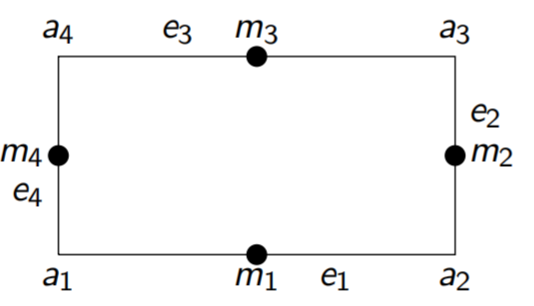
\includegraphics[width=0.7\linewidth]{rec}
			\label{fig:rec}
		\end{figure}
		
		\begin{proof}
			令$\xi=\frac{x-x_0}{\ell_1},\quad\eta=\frac{y-y_0}{\ell_2}.$
			
			考虑$v = \xi \eta$. 显然$v \in Q_1(K)$且$v(m_i)=0$,且$v \not\equiv 0$
		\end{proof}
		
		\item 如果 $K$ 是矩形, $P_K=\left\{1, x, y, \xi^2-\eta^2\right\}$, 证明 $\mathcal{N}_K=\left\{N_i, 1 \leq i \leq 4\right\}$,其中 $N_i(v)=\frac{1}{\left|e_i\right|} \int_{e_i} v \mathrm{ds}, 1 \leq i \leq 4$ 对 $P_K$ 是唯一可解的.
		
		\begin{proof}
			易得$P_K=\{1,\xi,\eta,\xi^2-\eta^2\}$,设$v = a_1 (\xi^2 - \eta^2) + a_2 \xi +a_3 \eta +a_4$.
			
			由$N_i(v) = 0, \quad i = 1,2,3,4$,可得
			$$\int_{-1}^1 -a_1 (1-\eta^2) + a_2 + a3\eta + a_4 d\eta =0$$
			$$\int_{-1}^1 -a_1 (1-\xi^2) + a_2 + a3\xi + a_4 d\xi =0$$
			$$\int_{-1}^1 -a_1 (1-\eta^2) - a_2 + a3\eta + a_4 d\eta =0$$
			$$\int_{-1}^1 -a_1 (1-\xi^2) - a_2 + a3\xi + a_4 d\xi =0$$
			
			即
			$$-\frac{2}{3}a_1+2(a_1+a_2+a_4)=0$$
			$$-\frac{2}{3}a_1+2(a_1+a_2+a_3)=0$$
			$$-\frac{2}{3}a_1+2(a_1-a_2+a_4)=0$$
			$$-\frac{2}{3}a_1+2(a_1-a_2+a_3)=0$$
			
			解得
			$$a_1=a_2=a_3=a_4 = 0$$
			
			从而$v \equiv 0$.
		\end{proof}
		\item 证明Morley有限元空间 $V_h$ 满足 $V_h \nsubseteq H^2(\Omega)$ 且 $V_h \nsubseteq H^1(\Omega)$
		
		Morley元的有限元空间:
		
		$V_h=\{v\in L^2(\Omega)\mid v|_K\in P_2(K),\forall K\in T_h,v$在$T_h$的所有顶点连续,
		$\frac{\partial v}{\partial\nu_\mathrm{e}}$在$\mathcal{T} _h$所 有 内 边 e的 中 点 连 续 $\}$
		
		\begin{proof}
			不妨设某条内边$e = (-1,0)\rightarrow(1,0)$,相邻单元为$K_1,K_2$.
			
			考虑$v |_ {K_1} = x^2-1,v |_ {K_2} = 1-x^2$.满足$v \in V_h$但$v \notin H^1(\Omega)$
		\end{proof}
		\item 验证课件中给出的函数是Morley元的节点基函数
		
		\begin{equation*}
			\begin{aligned}
				p_{i}=& 1-(\lambda_{i-1}+\lambda_{i+1})+2\lambda_{i-1}\lambda_{i+1}  \\
				&-\left(\nabla\lambda_{i-1}\right)^T\nabla\lambda_{i+1}\sum_{k=i-1,i+1}\frac{\lambda_k(\lambda_k-1)}{\left\|\nabla\lambda_k\right\|^2},\quad1\leq i\leq3 \\
				p_{i+3}=& \frac{\lambda_{i}(\lambda_{i}-1)}{\|\nabla\lambda_{i}\|},1\leq i\leq3. 
			\end{aligned}
		\end{equation*}
		
		\begin{equation*}
			\begin{aligned}
				N_i(v)=v(a_i),1\leq i\leq3\\N_{i+3}(v)=\frac{\partial v}{\partial\nu}(m_i),1\leq i\leq3
			\end{aligned}
		\end{equation*}
		
		$$a_1 = (1,0,0),a_2=(0,1,0),a_3=(0,0,1)$$
		$$m_1 = (0,0.5,0.5),m_2=(0.5,0,0.5),m_3=(0.5,0.5,0)$$
		
		\begin{proof}
			
			
			注意到$\nabla \lambda_i = \frac{1}{2|S_K|} (y_j-y_k,x_k-x_j)$,$e_i=(x_k-x_j,y_k-y_j)$.从而$-\nabla \lambda_i ^\top$为$e_i$ 的外法向量,$-\frac{\nabla \lambda_i}{\|\nabla \lambda_i\|}^\top$为$e_i$的单位外法向量$\nu_{e_i}$。
			
			$$N_1(p_1) = 1-(0+0)+2*0*0-0 = 0$$
			$$N_1(p_2) = 1- (1+0) - 2*1*0 - 0 = 0$$
			$$N_1(p_4) = \frac{0}{\|\nabla \lambda_1\|} = 0$$
			
			计算得
			$$
			\nabla p_{k}=\Big(-\nabla\lambda_i-\nabla\lambda_j+2(\lambda_i\nabla\lambda_j+\lambda_j\nabla\lambda_i)-\nabla\lambda_i^\top\nabla\lambda_j\sum_{k=i,j}\frac{(2\lambda_k-1)\nabla\lambda_k}{\|\nabla\lambda_k\|^2}\Big) \quad k = 1,2,3
			$$
			\begin{equation*}
				\begin{aligned}
					N_4(p_1) = \nabla p_1 (m_1) \cdot \nu_{e_1} = 0 \cdot \nu_{e_1} = 0
				\end{aligned}
			\end{equation*}
			\begin{equation*}
				\begin{aligned}
					N_4(p_2) &= \nabla p_2 (m_1) \cdot \nu_{e_1} \\
					&=\Big( -\nabla\lambda_{2}+\nabla\lambda_{1}^{\top}\nabla\lambda_{2}\frac{\nabla\lambda_{1}}{\|\nabla\lambda_{1}\|^{2} } \Big) \cdot  \Big(-\frac{\nabla \lambda_1}{\|\nabla \lambda_1\|}\Big)^\top\\
					&= 0.  (\text{利用单位外法向量})
				\end{aligned}
			\end{equation*}
			
			计算得
			$$\nabla p_{i+3}=\frac{1}{\|\nabla\lambda_i\|}(2\lambda_i-1)\nabla\lambda_i \quad i = 1,2,3$$
			\begin{equation*}
				\begin{aligned}
					N_4(p_4) = \nabla p_4(m_1) \cdot \nu_{e_1} = \Big(-\frac{\nabla \lambda_i}{\|\nabla \lambda_i\|}\Big)^\top\cdot \Big(-\frac{\nabla \lambda_i}{\|\nabla \lambda_i\|}\Big) = 1
				\end{aligned}
			\end{equation*}
			$$N_4(p_5) = \nabla p_5 (m_1) \cdot \nu_{e_1} = 0 \cdot \nu_{e_1} = 0$$
			
			结合对称性,验证完毕。
		\end{proof}
	\end{enumerate}
	
	\newpage
	
	\section*{2024.05.23}	
	
	\begin{enumerate}
		\item 证明二维单元$K$上迹定理
		$$\begin{aligned}&|e|^{-1}\|\xi\|_{0,e}^{2}\leq C\Big(h_{K}^{-2}\|\xi\|_{0,K}^{2}+|\xi|_{1,K}^{2}\Big),\:\forall\xi\in H^{1}(K)\end{aligned}$$
		Hint: 利用仿射变换以及尺度(scailing)技巧
		
		\begin{proof}
			考虑参考单元$\hat{K}$,满足$|\hat{e}|=1$.
			
			\begin{equation*}
				\begin{aligned}
					C(\|\hat{\xi}\|_{0,\hat{K}}^{2}+|\hat{\xi}|_{1,\hat{K}}^{2}) = C\|\hat{\xi}\|_{1,\hat{K}}^2 \geq \|\hat{\xi}\|^2_{0,\hat{e}} = \int_{\hat{e}} \hat{\xi}^2 d\hat{s} = \int_{e}  \xi^2 \frac{|\hat{e}|}{|e|} ds = |e|^{-1}\|\xi\|_{0,e}^{2} 
				\end{aligned}
			\end{equation*}
			
			结合尺度变换关系以及
			
			$$
			|\hat{v}|_{m,p,\hat{K}}\leq C\left\|B\right\|^m|\mathrm{det}B|^{-1/p}|v|_{m,p,K}
			$$
			
			代入$p = 2, m= 2$即得证.
			
		\end{proof}
		
		\item 对于一维单元e证明
		$$\begin{aligned}\left\|\xi-P_{e}^{0}\xi\right\|_{0,e}&\leq\frac{|e|}\pi|\xi|_{1,e}\:,\:\forall\xi\in H^1(e)\\\left\|\xi\right\|_{0,e}&\leq\frac{|e|}\pi|\xi|_{1,e}\:,\:\forall\xi\in H_0^1(e)\end{aligned}$$
		
		Hint:考虑特征值问题 $-\frac{\partial^2 \xi}{\partial s^2} = \lambda \xi$在$\xi \in H^1(e)$和$\xi \in H_0^1(e)$的特征函数以及最小特征值
		
		\begin{proof}
			
			只需证第二个式子,不妨设一维单元$e = [0,L]$.
			
			考虑$-\xi ^{\prime\prime} = \lambda \xi, \xi(0) = \xi(L) = 0$的特征值$\lambda = \displaystyle \frac{n^2 \pi^2}{L^2} , n \in \mathbb{Z^*}$.
			
			有
			
			$$\int_0^L - \xi^{\prime\prime} \xi d\xi =\lambda \int_0^L \xi^2 d\xi$$
			分部积分
			$$\int_0^L (\xi^{\prime})^2 d\xi  =\lambda \int_0^L \xi^2 d\xi  $$
			$$\lambda \|\xi\|_{0,e}^2 = |\xi|_{1,e}^2$$
			
			注意到最小特征值$\lambda = \frac{\pi^2}{L^2}$,进而
			
			$$\frac{\pi^2}{L^2} \|\xi\|_{0,e}^2 \leq |\xi|_{1,e}^2$$
			
		\end{proof}
		
		
		
		\item 证明
		$$\|v-P_ev\|_{0,e}=\inf_{c\in\mathbb{R}}\|v-c\|_{0,e}$$
		
		\begin{proof}
			
			$$\begin{aligned}
				\|v-P_e v\|_{0,e}^2 &= \int_e \left(v-\frac{1}{|e|}(\int_e v ds)^2\right)ds\\
				& = \int_e v^2 ds - \frac{1}{|e|}(\int_e v ds)^2\\
				& \geq \int_e v^2 ds - 2c \int_e v ds + c^2 |e| \qquad \text{(均值不等式)}\\
				& = \int_e (v-c)^2 ds\\
				& = \|v-c\|_{0,e}^2
			\end{aligned}$$
			
		\end{proof}
		
		\item 证明Morley元的$H^{1}$范数误差估计
		
		\begin{proof}
			令$\Pi_{h_0}^p,\Pi_{h_0}^{p,2}$为一次Lagrange元与二次Lagrange元的协调元插值算子. 记$w_h = \Pi_{h_0}^p u$.
			
			由协调元插值误差估计以及庞加莱不等式,有
			\begin{equation}\label{eq1}
				\begin{aligned}
					\begin{aligned}\|u-u_h\|_{1,h}\end{aligned}& \leqslant\|u-w_h\|_{1,h}+\|\Pi_{h0}^{p,2}(w_h-u_h)\|_{1,\Omega}  \\
					&+\|w_h-u_h-\Pi_{h0}^{p,2}(w_h-u_h)\|_{1,h} \\
					&\lesssim|u-w_h|_{1,h}+h|w_h-u_h|_{2,h}+\|\Pi_{h0}^{p,2}(w_h-u_h)\|_{1,\Omega} \\
					&\lesssim h^2|u|_{3,\Omega}+\|\Pi_{h0}^{p,2}(w_h-u_h)\|_{1,\Omega},
				\end{aligned}
			\end{equation}
			
			
			
			下面估计$\|\Pi_{h0}^{p,2}(w_h-u_h)\|_{1,\Omega}$,注意到:
			
			\begin{equation}\label{eq2}
				\|\Pi_{h0}^{p,2}(w_h-u_h)\|_{1,\Omega}=\sup_{0\neq g\in L^2(\Omega)}\frac{|(g,\Pi_{h0}^{p,2}(w_h-u_h))|}{\|g\|_{-1,\Omega}}
			\end{equation}
			
			
			只需估计$|(g,\Pi_{h0}^{p,2}(w_h-u_h))|$, 对$g\in L^2(\Omega)$,令$\phi_g\in H_0^2(\Omega)$和$\phi_{gh}\in V_{h_0}$分别是下面问题的解:
			$$a(v,\phi_g)=(g,v),\quad\forall v\in H_0^2(\Omega),$$
			
			$$a_h(v_h,\phi_{gh})=(g,\Pi_{h0}^{p,2}v_h),\quad\forall v_h\in V_{h0}.$$
			
			
			由$H^2$范数误差估计以及椭圆方程正则性结果,得
			
			\begin{equation}\label{eq3}
				|\phi_g-\phi_{gh}|_{2,h}\lesssim h|\phi_g|_{3,\Omega},\quad\|\phi_g\|_{3,\Omega}\lesssim\|g\|_{-1,\Omega}
			\end{equation}
			
			
			我们有
			$$
			\begin{aligned}
				(g,\Pi_{h0}^{p,2}(w_h-u_h))& \begin{aligned}=a_h(w_h-u_h,\phi_{gh})\end{aligned}  \\
				&=a_h(u-w_h,\phi_g-\phi_{gh})+\left(a_h(u,\phi_{gh}-\phi_g)-(f,\phi_{gh}-\phi_g)\right) \\
				&+\Big(a_h(w_h-u,\phi_g)-(g,\Pi_{h0}^{p,2}(w_h-u))\Big)+(g,\Pi_{h0}^{p,2}(w_h-u)).
			\end{aligned}
			$$
			
			下面只需要对上式右侧的四项分别估计:
			
			\textbf{对第一项},由算子有界性、协调元插值误差以及\eqref{eq3},有
			
			\begin{equation}\label{eq4}
				|a_h(u-w_h,\phi_g-\phi_{gh})|\lesssim h^2|u|_{3,\Omega}\|g\|_{-1,\Omega}.
			\end{equation}
			\textbf{对第四项},有
			$$|(g,\Pi_{h0}^{p,2}(w_h-u))|\lesssim\|g\|_{-1,\Omega}\|\Pi_{h0}^{p,2}(w_h-u)\|_{1,\Omega}.$$
			由逆不等式与插值误差估计,有
			$$\begin{aligned}|\Pi_{h0}^{p,2}(w_{h}-u)|_{1,\Omega}^{2}&=\sum_{T\in T_{h}}|\Pi_{h0}^{p,2}(w_{h}-u)|_{1,T}^{2}\\&\lesssim\sum_{T\in T_{h}}h_{T}^{-2}|\Pi_{h0}^{p,2}(w_{h}-u)|_{0,T}^{2}\\&\lesssim\sum_{T\in T_{h}}h_{T}^{-2}|w_{h}-u|_{0,T}^{2}\lesssim h^{4}|u|_{3,\Omega}^{2},\end{aligned}$$
			再利用庞加莱不等式,得到
			\begin{equation}\label{eq5}
				\|\Pi_{h0}^{p,2}(w_h-u)\|_{1,\Omega}\lesssim h^2|u|_{3,\Omega}
			\end{equation}
			
			\textbf{对第二项},记
			$$e_{h1}=\phi_{gh}-\Pi_{h0}^p\phi_g,\quad e_{h2}=\Pi_{h0}^p\phi_g-\phi_g,$$
			则
			$$a_h(u,\phi_{gh}-\phi_g)-(f,\phi_{gh}-\phi_g)$$
			$$=\sum_{i=1}^2\Big(a_h(u,e_{hi})-(f,\Pi_{h0}^pe_{hi})-(f,e_{hi}-\Pi_{h0}^pe_{hi})\Big).$$
			令$i\in\{1,2\}.$由Morley元相容项误差估计,有
			$$\left|a_h(u,e_{hi})-(f,\Pi_{h0}^{p,2}e_{hi})\right|\lesssim|u|_{3,\Omega}\left(h|e_{hi}|_{2,h}+|e_{hi}-\Pi_{h0}^{p,2}e_{hi}|_{1,h}\right).$$
			另一方面,
			$$|(f,e_{hi}-\Pi_{h0}^{p,2}e_{hi})|\lesssim\|f\|_{0,\Omega}\|e_{hi}-\Pi_{h0}^{p,2}e_{hi}\|_{0,\Omega}.$$
			由协调元误差估计,得到
			$$\|e_{h1}-\Pi_{h0}^{p,2}e_{h1}\|_{0,\Omega}+h\|e_{h1}-\Pi_{h0}^{p,2}e_{h1}\|_{1,h}\lesssim h^2|e_{h1}|_{2,h}.$$
			对于$e_{h2}$,类似于式\eqref{eq5} 有
			$$\|\Pi_{h0}^{p,2}e_{h2}\|_{1,\Omega}\lesssim h^2|\phi_g|_{3,\Omega}.$$
			由协调元插值误差,有
			$$|e_{h2}|_{1,\Omega}\lesssim h^2|\phi_g|_{3,\Omega}.$$
			$$\|e_{h2}-\Pi_{h0}^{p,2}e_{h2}\|_{0,\Omega}\lesssim\|e_{h2}\|_{0,\Omega}\lesssim h^3|\phi_g|_{3,\Omega}.$$
			总结上面的讨论得到
			$$|a_h(u,\phi_{gh}-\phi_g)-(f,\phi_{gh}-\phi_g)|\lesssim h^2(|u|_{3,\Omega}+h\|f\|_{0,\Omega})|\phi_g|_{3,\Omega}.$$
			结合\eqref{eq3},得到
			\begin{equation}\label{eq6}
				|a_h(u,\phi_{gh}-\phi_g)-(f,\phi_{gh}-\phi_g)|\lesssim h^2(|u|_{3,\Omega}+h\|f\|_{0,\Omega})\|g\|_{-1,\Omega}
			\end{equation}
			\textbf{对第三项},与第二项做类似讨论可得
			\begin{equation}\label{eq7}
				|a_h(w_h-u,\phi_g)-(g,\Pi_{h0}^{p,2}(w_h-u))|\lesssim h^2|u|_{3,\Omega}\|g\|_{-1,\Omega}.
			\end{equation}
			
			结合式\eqref{eq1}\eqref{eq2}\eqref{eq3}\eqref{eq5}\eqref{eq6}\eqref{eq7},得到Morley元$H^1$误差估计:
			$$
			\|u-u_h\|_{1,h}\lesssim h^2\left(|u|_{3,\Omega}+h\|f\|_{0,\Omega}\right).
			$$
		\end{proof}
	\end{enumerate}
	
	\newpage
	
		\section*{2024.05.27}	
	
	\begin{enumerate}
		\item 证明Poisson问题的混合变分形式的弱解在一定光滑条件下是古典解
		
		Poisson问题:
		$$\begin{cases}
			\mathbf{p} - \nabla u = 0 \\
			div \mathbf{p} = - f \\
			u |_{\partial \Omega} = 0
		\end{cases}$$
		
		混合变分形式:
		求$(\mathbf{p},u)\in H(\mathrm{div},\Omega)\times L^2(\Omega)$,使
		
		$$\begin{cases}
			\int_\Omega \mathbf{p}\cdot\mathbf{q} dx + \int_\Omega div\mathbf{q} u dx= 0,\quad \forall \mathbf{q} \in H(\mathrm{div},\Omega) \\
			\int_\Omega div\mathbf{p} v dx= \int_\Omega -f v dx,\quad \forall v \in L^2(\Omega)
		\end{cases}$$
		
		\begin{proof}
			当解足够光滑,由$	\int_\Omega div\mathbf{p} v = \int_\Omega -f v dx,\quad \forall v \in L^2(\Omega) $,有
			
			$$	\int_\Omega (div\mathbf{p} + f) v dx =0 ,\quad \forall v \in L^2(\Omega)$$
			
			由$v$的任意性,得到$div\mathbf{p} + f = 0$.即$div\mathbf{p} = -f$.
			
			在$\int_\Omega \mathbf{p}\cdot\mathbf{q} dx + \int_\Omega div\mathbf{q} u dx= 0$中取$\forall \mathbf{q} \in H(\mathrm{div},\Omega) \cap (H_0^1(\Omega))^2$,得到
			
			$$\int_{\Omega} \mathbf{q}\cdot(\mathbf{p}-\nabla u) dx= 0$$
			
			由$\mathbf{q}$的任意性,得到$	\mathbf{p} - \nabla u = 0$.
			
			再在$\int_\Omega \mathbf{p}\cdot\mathbf{q} dx + \int_\Omega div\mathbf{q} u = 0$中取$\forall \mathbf{q} \in H(\mathrm{div},\Omega)$,得到
			
			$$\int_{\partial \Omega} u \mathbf{q}\cdot\mathbf{n} ds= 0$$
			
			由$\mathbf{q}$的任意性,得到$	u |_{\partial \Omega} = 0$.
		\end{proof}
		\item 推导Stokes问题的混合变分形式
		
		
		Stokes问题:
		
		$$\begin{cases}-\Delta\mathbf{u}+\nabla p=\mathbf{f},\text{在}\Omega\text{内}\\\operatorname{div}\mathbf{u}=0,\text{在}\Omega\text{内}\\\mathbf{u}|_{\partial\Omega}=0\end{cases}$$
		
		\begin{proof}
			在$-\Delta\mathbf{u}+\nabla p=\mathbf{f}$中,对$\forall \mathbf{v} \in (H_0^1(\Omega))^2$有
			
			$$\int_\Omega -\Delta \mathbf{u} \cdot \mathbf{v} + \nabla p \mathbf{v} dx = \int_{\Omega} \mathbf{f} \mathbf{v} dx$$
			
			利用两次Green公式和$\mathbf{v}|_{\partial\Omega}=\frac{\partial \mathbf{v}}{\partial \mathbf{n}}|_{\partial\Omega}=0$以及散度积分公式可得
			
			$$\int_\Omega \nabla \mathbf{u} : \nabla \mathbf{v} + div\mathbf{v} p  dx = \int_{\Omega} \mathbf{f} \mathbf{v} dx$$
			
			在$div\mathbf{u}=0$中,对$\forall q \in L_0^2(\Omega)$,有
			
			$$\int_{\Omega} div\mathbf{u} q dx = 0$$
			
			得到混合变分形式.
		\end{proof}
		\item 证明inf-sup条件的定理中(3)等价于(1)和(2). 
		
		\begin{proof}
			已有(1) $\Leftrightarrow$ (2).
			
			(2) $\Rightarrow$ (3):
			
			假设 (2) 成立,则对给定的$u\in U^\perp$,定义函数$g\in U^\prime$如下
			
			
			\begin{equation}\tag{$\ast$} \label{EQ1}
				g(w)=(u,w),\quad\forall w\in U
			\end{equation}
			
			容易验证$g\in U^0$,又因为$B^\prime$是$V$到$U^0$的同构,故存在$\lambda\in V$,使
			
			\begin{equation}\tag{$\star$} \label{EQ2}
				b(w,\lambda)=(w,B'\lambda)=g(w)
			\end{equation}
			
			又由$\eqref{EQ1}$易证$||g||_{U^{\prime}}=||u||_{U}$,从而
			$$||u||_U=||g||_{U'}=||B'\lambda||_{U'}\geq\beta||\lambda||_V.$$
			
			在$\eqref{EQ2}$中令$w=u$,则有
			$$\sup\limits_{v\in V}\frac{b(u,v)}{||v||_V}\geq\frac{b(u,\lambda)}{||\lambda||_V}=\frac{(u,u)}{||\lambda||_V}\geq\beta||u||_U,$$
			从而$B:U^{\perp}\to V^{\prime}$满足Babuška定理的三个条件,故$B$是一个同构映射.
			
			(3) $\Rightarrow$ (1):
			
			因 (3) 成立,故$B:U^\perp\to V^{\prime}$是一个同构,对给定的$v\in V$,
			$$\begin{aligned}||v||_{V}&=\sup_{g\in V^{\prime}}\frac{\langle g,v\rangle}{||g||_{V^{\prime}}}=\sup_{u\in U^{\perp}}\frac{\langle Bu,v\rangle}{||Bu||_{V^{\prime}}}\\&=\sup_{u\in U^{\perp}}\frac{b(u,v)}{||Bu||_{V^{\prime}}}\leq\sup_{u\in U^{\perp}}\frac{b(u,v)}{\beta||u||_{U}}\leq\frac{1}{\beta}\sup_{u\in U}\frac{b(u,v)}{||u||_{U}},\end{aligned}$$
			从而 (1)成立,证毕.
			
			
		\end{proof}
		\item 如果$\dim U_h= \dim V_h$, 离 散 的 inf-sup条 件 
		$$\inf_{u_h\in U_h}\sup_{v_h\in V_h}\frac{b(u_h,v_h)}{\|u_h\|_U\|v_h\|_V}=\beta_h>0$$
		成立.说明离散问题:求$u_h\in U_h$使得
		$$b(u_h,v_h)=\langle f,v\rangle_{V^{\prime}\times V}$$
		存在唯一解.
		
		(注:该结果说明对于离散问题只需验证Babuška定理中(b)对应的离
		散形式和维数相等,无需验证(c)的离散形式) 
		
		\begin{proof}
			定义算子$B$以及对偶算子$B^\prime$
			$$
			B:U\to V^{\prime}<Bu,v>_{V^{\prime}\times V}=b(u,v)\quad\forall u\in U,v\in V$$
			$$B^{\prime}:V\to U^{\prime}<B^{\prime}v,u>_{U^{\prime}\times U}=b(u,v)\quad\forall u\in U,v\in V.
			$$
			
			当$\dim U= \dim V$时,根据闭值域定理,算子$B$有连续逆算子${B}^{-1} :V^\prime \rightarrow U$,$B^\prime$有连续逆算子${(B^\prime)}^{-1} :U^\prime \rightarrow V$,满足
			
			$$
			\|(B')^{-1}\|=\|(B^{-1})'\|=\|B^{-1}\|
			$$
			
			从而有
			
			$$\inf_{u_h\in U_h}\sup_{v_h\in V_h}\frac{b(u_h,v_h)}{\|u_h\|_U\|v_h\|_V}=\inf_{v_h\in V_h}\sup_{u_h\in U_h}\frac{b(u_h,v_h)}{\|u_h\|_U\|v_h\|_V}=\beta_h>0$$
			
			从而(b)与(b')成立,进而可以推出(b)与(c)成立.
			
		\end{proof}
		\item 证明$H(div,\Omega)$空间在范数$\|\cdot\|_{div,\Omega}$下是完备的
		
		$$\|\cdot\|_{div,\Omega} \coloneqq (\|\cdot\|_{L^2(\Omega)}^2 + \|div(\cdot)\|_{L^2(\Omega)}^2)^{\frac{1}{2}}$$
		
		\begin{proof}
			设 $\{u_m=(u^1,\cdots,u^n)\}_{m\in\mathbb{N}}$ 是 $(H(div,\Omega),\|\cdot\|_{div,\Omega})$ 中的Cauchy列。
			
			对于 $i\in\{1,\cdots,n\}$,有
			
			$$(u_m^i-u_l^i,u_m^i-u_l^i)=\left\|u_m^i-u_l^i\right\|_{L^2(\Omega)}^2\leq\left\|u_m-u_l\right\|_{div,\Omega}^2$$
			
			由于$\{u_m\}_{m\in\mathbb{N}}$是$(H(div,\Omega),\|\cdot\|_{div,\Omega})$ 中的Cauchy列,有 $\{u_m^i\}_{m\in\mathbb{N}}$ 是 $L^2(\Omega)$ 中的Cauchy列。由于 $L^2(\Omega)$ 的完备性,有 $u_m^i\to u^i\in L^2(\Omega), \quad m\to\infty$.因此$u=(u^1,\cdots,u^n)\in\{L^2(\Omega)\}^n$
			
			类似地,
			$$
			(\mathrm{div}\:(u_m-u_l),\mathrm{div}\:(u_m-u_l))_{L^2(\Omega)}=\left\|\mathrm{div}\:u_m-\mathrm{div}\:u_l\right\|_{L^2(\Omega)}^2\leq\left\|u_m-u_l\right\|_{H(div,\Omega)}^2
			$$
			因此 $\{\mathrm{div} \:u_m\}_{m\in\mathbb{N}}$ 在 $L^2(\Omega)$ 中是Cauchy列。由于 $L^2(\Omega)$ 的完备性,有$\mathrm{div} u_m\to g\in L^2(\Omega), \quad m\to\infty$
			
			下面只需要说明$div u = g$,这等价于证明$\int_\Omega g\phi dx=-\int_\Omega u\cdot\nabla\phi dx,\quad \forall \phi\in C_0^\infty(\Omega).$
			
			事实上,只需注意到
			
			$$\int_{\Omega}\phi\operatorname{div}u_{m} dx=-\int_{\Omega}u_{m}\cdot\nabla\phi dx.$$
			$$\operatorname{div}u_{m}\to g\mathrm{~in~}\|\cdot\|_{L^{2}(\Omega)}\implies\int_{\Omega}\phi\operatorname{div}u_{m} dx\to\int_{\Omega}\phi g dx$$
			$$u_{m}\to u\mathrm{~in~}\|\cdot\|_{L^{2}(\Omega)}\implies\int_{\Omega}u_{m}\cdot\nabla\phi dx\to\int_{\Omega}u\cdot\nabla\phi dx.$$
			
			即可得到。
		\end{proof}
		
		
	\end{enumerate}
	
	\newpage
	
	\section*{2024.06.03}	
	
	\begin{enumerate}
		
		\item 验证Stokes问题的inf-sup条件证明中$\mathbf{v}_2$满足
		$$\mathrm{div} \mathbf{v}_2=0,\:\mathbf{v}_2\cdot\nu|_{\partial\Omega}=0,\:\mathbf{v}_2\cdot\tau|_{\partial\Omega}=-\mathbf{v}_1\cdot\tau|_{\partial\Omega}$$
		
		\begin{proof}
			$$\mathrm{div} \  \mathbf{v}_2 = \mathrm{div} \ \mathrm{curl} \psi = \frac{\partial^2 \psi}{\partial x_1 \partial x_2} - \frac{\partial^2 \psi}{\partial x_2 \partial x_1} = 0  $$
			$$\mathbf{v}_2\cdot\nu|_{\partial\Omega}=\mathrm{curl} \cdot \nu|_{\partial \Omega}=\nabla \psi \cdot \tau |_{\partial \Omega}=\frac{\partial \psi}{\partial \tau} |_{\partial\Omega}=0$$
			$$\mathbf{v}_2\cdot\tau|_{\partial\Omega}=\mathrm{curl} \psi \cdot \tau|_{\partial\Omega}=\nabla \psi \cdot \nu |_{\partial\Omega}=- \frac{\partial \psi}{\partial \nu}|_{\partial \Omega}=-\mathbf{v}_1\cdot\tau|_{\partial\Omega}$$
		\end{proof}
		
		\item 证明在$P_2-P_0$元分析中构造的插值算子$\Pi_h^{2}$满足以下三条性质
		
		\begin{enumerate}
			\item $\Pi _{h}^{2}v\in H_{0}^{1}( \Omega )$, $\forall v\in H_{0}^{1}( \Omega )$
			
			\begin{proof}
				由$v \in H^1(\Omega)$,可得$\Pi_h^2 v$在公共边两个端点处连续(=0),在公共边积分值连续($\int_{e_i} \Pi_h^2 v ds= \int_{e_i} v ds$).
				
				由$\Pi_h^2 v|_K \in P_2(K)$,可得$\Pi_h^2 v$在公共边上连续,即$\Pi_h^2 v \in H^1(\Omega)$.
				
				类似的,由$v \in H_0^1(\Omega)$,可得$\Pi_h^2 v$在边界为0,即$\Pi_h^2 v \in H_0^1(\Omega)$.
			\end{proof}
			
			\item $ \left \| \Pi _h^2v\right \| _{0, K}\leq C\left ( \left \| v\right \| _{0, K}+ h_K\left | v\right | _{1, K}\right )$, $\forall v\in H_0^1( \Omega )$.
			
			\begin{proof}
				通过尺度变换技巧变换到参考单元:
				$$|\Pi_{h}^2{v}|_{1,K}=|\widehat{\Pi_{h}^2{v}}|_{1,\hat{K}}\leq C||\hat{v}||_{1,\hat{K}}\leq C(h_{K}^{-1}|{v}|_{0,K}+|{v}|_{1,K}).$$
				再利用逆估计得到结果.
			\end{proof}
			
			\item $b(\Pi_h^2\mathbf{v},q_h)=b(\mathbf{v},q_h),\:\forall q_h\in Q_h$
			
			\begin{proof}
				由$\Pi_h^2 v$的定义有
				\begin{equation*}
					\begin{aligned}
						&\int_e (v-\Pi^2_h v) \cdot \nu q_h ds=0,\quad \forall q_h \in Q_h, \quad \forall e \in \partial K \\
						\Rightarrow & \int_{\partial K} (v-\Pi^2_h v) \cdot \nu q_h ds=0 ,\quad \forall q_h \in Q_h\\
						\Rightarrow & \int_K \mathrm{div}(v-\Pi^2_{h}v) q_h dx = 0,\quad \forall q_h \in Q_h, \quad \forall K \subset \Gamma_h \\
						\Rightarrow & \int_{\Omega} \mathrm{div}(v-\Pi^2_{h}v) q_h dx = 0,\quad \forall q_h \in Q_h \\
						\Rightarrow & b(v-\Pi^2_{h}v,q_h) = 0,\quad \forall q_h \in Q_h		
					\end{aligned}
				\end{equation*}
				
			\end{proof}
		\end{enumerate}
		
		\item 证明Stokes离散问题的分析中构造的Fortin插值$\Pi_h$满足误差估计
		$$\left\|\mathbf{u}-\Pi_h\mathbf{u}\right\|_{1,\Omega}\leq Ch\left|u\right|_{2,\Omega}$$
		思考当$u\in H^3(\Omega)$时,是否有
		$$\left\|\mathbf{u}-\Pi_h\mathbf{u}\right\|_{1,\Omega}\leq Ch^2\left|u\right|_{3,\Omega}$$
		
		\begin{proof}
			$$u - \Pi_h u = u- \Pi_h^1 u - \Pi_h^2(u-\Pi_h^1 u)$$
			其中$\Pi_h^1$ 为Scott-Zhang插值.有
			$$\|u-\Pi_h u\|_{1,\Omega}\leq\|u-\Pi_h^1 u\|_{1,\Omega}+\|\Pi_h^2 (u-\Pi_h^1 u)\|_{1,\Omega}$$
			对于第一项,利用Scott-Zhang插值误差结果
			$$\|u-\Pi_h^1 u\|_{1,\Omega} \leq ch|u|_{2,\Omega}$$
			对第二项,利用逆估计
			$$\|\Pi_h^2 (u-\Pi^1_u)\|_{1,K} \leq C h_K^{-1} \|\Pi_h^2(u-\Pi_h^1 u)\|_{0,K} \leq Ch_K^{-1}(\|u-\Pi_h^1 u\|_{0,K}+h_K|u-\Pi_h^1 u|_{1,K}) $$
			再利用Scott-Zhang插值误差结果
			$$\|u-\Pi_h^1 u\|_{0,\Omega}\leq Ch^2|u|_{2,\Omega}$$
			故$$\|\Pi_h^2 (u-\Pi_h^1 u)\|_{1,\Omega}\leq Ch|u|_{2,\Omega}$$
			因此
			$$\left\|u-\Pi_h u\right\|_{1,\Omega}\leq Ch\left|u\right|_{2,\Omega}$$
			
			当$u\in H^3(\Omega)$时,证明方法类似.
			
		\end{proof}
		\item 证明$P_1-P_0$元不满足离散的LBB条件.(Hint: 可通过数维数的方法
		导出这时$\dim V_h < \dim Q_h$,从而说明存在$q_h\in Q_h$使
		得$b(v_h,q_h)=0.\forall v_h\in V_h)$	
		
		\begin{proof}
			对于给定的剖分,记$t$为三角形数量,$v_I$为内部顶点数量,$v_B$为边界顶点数量.由欧拉公式,有$t=2v_I+v_B-2$.
			
			由空间定义,我们有$\dim V_h = 2 v_I, \dim Q_h = t-1$.
			
			定义算子$B_h:V_h\rightarrow {Q_h}^\prime$,使得$\int_{\Omega}(B_h({v}_h)-\nabla\cdot{v}_h)q_h {d}x=0, \quad \forall q_h \in Q_h$,并记其对偶算子为$B_h^\top:Q_h \rightarrow {V_h}^\prime$.
			
			当$v_B > 3$时,有
			$$\dim(\ker(B_h^\top)) =\dim(Q_{h})-\dim(\mathrm{im}(B_{h}^{\top}))\geq\dim(Q_{h})-\dim(V_{h})=t-1-2v_I=v_B-3>0$$
			
			从而存在$q_h\in Q_h$使
			得$b(v_h,q_h)=0.\forall v_h\in V_h$	
		\end{proof}
		
	\end{enumerate}
	
\end{document}

